% Chapter 1

\chapter{\color{thesisBlue} Relating Neural Data to Stimulus Parameters in 3+ Dimensions} % Main chapter title

\label{ch:optim} % For referencing the chapter elsewhere, use \ref{Chapter1} 

%----------------------------------------------------------------------------------------

% Define some commands to keep the formatting separated from the content 
\newcommand{\keyword}[1]{\textbf{#1}}


%----------------------------------------------------------------------------------------
%	Chapter intro
%----------------------------------------------------------------------------------------
In this section I will introduce various analysis approaches for quantifying neural population tuning to stimulus spaces of arbitrary dimensionality. These approaches will first be applied to a simulated population of neurons in order to build intuition for the neural data in chapter \ref{ch:maps}.


%----------------------------------------------------------------------------------------
%	3D NEURON SIMULATION SECTION
%----------------------------------------------------------------------------------------


\section{Simulated Neural Populations}
\label{sec:ccaSimulations}
I begin by referring back to the 1D tuning curve from chapter \ref{ch:intro}, figure \ref{fig:tuningIntro}. I use the simple gaussian tuning curve as a template, and apply it to a small population of 3 neurons along 3 arbitrary stimulus dimensions. The choice of 3D neural state space and 3D stimulus space comes from the curse of dimensionality; in order to completely sample the spaces, 3 dimensions is the maximum due to combinatorics. For the sake of simplicity I will begin with a set of axioms with which to constrain my artificial neurons:

\begin{enumerate}
	\item \label{ax:bounds} Neurons have a minimum ($0$) and maximum ($R_{max}$) firing rate 
	\item \label{ax:gauss} Neurons are gaussian tuned to each stimulus dimension.
	\item There is one global maximum stimulus per neuron, which lies at a point in the stimulus space ($\harpoon{\rho_n}$).
	\item \label{ax:distfx} Neurons' responses to stimuli is some function of distance between its' preference and the stimuli
	\item Tuning to each stimulus dimension is independent of other dimensions (e.g. color and orientation tuning are assumed independent).
	\item \label{ax:nocorr} Neurons' responses to stimuli are independent from other neurons
\end{enumerate}

Later on, I will reduce the number of assumptions by adding in neural correlations and tuning dependence, but for now start with the simplest model. 

\subsection{Defining the Population Response Function}

Due to axiom \ref{ax:nocorr}, I can calculate the responses of each neuron independently and define a single response function $f_n(\harpoon\theta)$. This function is bounded by $f_n(\harpoon\theta) \in [0, R_{max}]$ according to axiom \ref{ax:bounds}. If we combine axioms \ref{ax:gauss} and \ref{ax:distfx} with these natural boundaries, we get equation \ref{eq:response}, which defines the neural response in terms of the stimulus values ($\harpoon\theta$), peak firing rate ($R_{max}$), and decay term ($D_n(\harpoon\theta)$; i.e. tuning width) for a stimulus space of arbitrary dimensionality.

\begin{equation}
	\label{eq:response}
	f_n(\harpoon{\theta}) = R_{max} \cdot e^{D_n(\harpoon\theta)}
\end{equation}

The decay term, ${D_n(\harpoon\theta)} \in [-\infty, 0]$, depends on both the euclidean distance between $\harpoon\theta$ and $\harpoon{\rho_n}$, and the neurons' tuning matrix ($\tau_n$). $\tau_n$ determines the rate at which the firing rate decays as $\harpoon\theta$ diverges from $\harpoon{\rho_n}$.

\begin{equation}
	\label{eq:decay}
	D_n(\harpoon\theta) = (\harpoon{\rho_n} -\harpoon\theta)^\top \cdot \tau_n \cdot (\harpoon\theta-\harpoon{\rho_n})
\end{equation}

Neurons therefore respond maximally to their preferred stimulus $\harpoon{\rho_n}$ at a rate of $R_{max}$. As the stimulus parameters differ along any dimension, this maximum response decays exponentially at a rate defined by $\tau_n$.

\begin{table}
	\centering
	\begin{tabular}{|c|c|}
		\hline
		\textbf{Symbol}       & \textbf{Description} \\
		\hline
		$\harpoon\theta$      & Vector of stimulus values for presented stimulus \\
		$\harpoon{\rho_n}$    & Vector of preferred stimulus values for neuron $n$ \\
		$f_n(\harpoon\theta)$ & Response in $\frac{spk}{s}$ for neuron $n$ to stimulus $\harpoon\theta$ \\
		$D_n(\harpoon\theta)$ & Decay term for neuron $n$ to stimulus $\harpoon\theta$ \\
		$R_{max}$             & Maximum firing rate \\
		$\tau_n$              & Tuning matrix for neuron $n$ \\
		\hline
	\end{tabular}
	\label{tbl:symbols}
\end{table}


\subsection{Deterministic Simulations}
\glsreset{cca}
If we ignore for the moment neural response variability, we can analyze the expected values of the population response in stimulus space. I begin with a relatively simple approach to quantifying linear relationships between the two 3D spaces, \gls{cca}. \gls{cca} rotates the two spaces and orders the new bases by descending correlation. In this way, I can pull out which stimulus dimension is most linearly related to the neural dimensions (CCA pair 1). This answers the question: "which stimulus dimension is best at predicting neural responses." A variety of neural parameters will ultimately affect these relationships, which I will expand on in this section. 

\begin{figure}
	\centering
	\includegraphics[width=100mm]{tuningWidthSimulationFigure.pdf}
	\caption{The effect of tuning width on \gls{cca}.}{Top row.) Example tuning curves for three simulations with descending tuning widths. First column.) Canonical correlation variable pairs for a population of 3 neurons with wide tuning. Neurons were assumed to have the same tuning width but different preferred stimuli along the three dimensions. Second\&Third column.) Same as first column but for medium and narrow tuning respectively.}
	\label{fig:ccaTuning}
\end{figure}

we can see clearly from figure \ref{fig:ccaTuning}, as tuning narrows for a neural population the correlations drop significantly. One way to interpret this is that a linear-readout of stimulus encoding is only possible in the wide-tuning regime. Once the neural data becomes too "peaky" (neurons respond profoundly to a single stimulus but weakly to most stimuli), a linear approach is no longer appropriate. In real-world situations this is not an issue. As discussed previously, natural visual scenes contain innumerable variability and dimensionality, and as the dimensionality of a stimulus increases, wider tuning is known to be more effective at conveying accurately and robustly \parencite{Brown2006}.

Another important feature of neurons that can affect these analyses is the dimensionality of the neural tuning space relative to the dimensionality of the stimulus space. In a naturalistic setting, there will undoubtedly be stimulus features that neurons are not tuned to. For example, if color is present for a purely orientation-tuned neuron, or visual features in general for an auditory neuron. When working in 10+ feature dimensions, having stimulus variability that is irrelevant for neurons allows for \gls{cca} to capitalize on the extra dimensionality. This becomes clear in figure \ref{fig:ccaInvarDim}, where the embedding dimensionality remains the same across models but the dimensionality of tuning decreases. As the number of relevant stimulus dimensions for neurons decreases, the $R^2$ for the tuned variables increases.

\begin{figure}
	\centering
	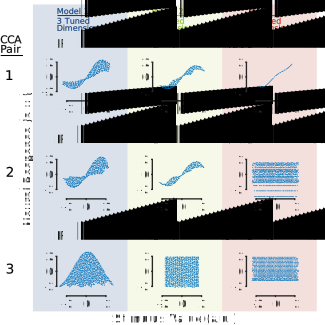
\includegraphics[width=100mm]{invariantDimSimulationFigure.pdf}
	\caption{The effect of irrelevant stimulus dimensions on CCA.}{Canonical correlation variable pairs for three models relating neural population space to stimulus space. Model 1.) Similar to models shown in figure \ref{fig:ccaTuning}, with all three stimulus dimensions being relevant to the neurons. Tuning for neurons was set at 50 a.u. across models. Model 2.) Same as model 1, except one stimulus parameter (consistent across neurons) was set to have no impact on the firing rate of the neurons. Model 3.) Same as model 2 but with multiple irrelevant stimulus dimensions.}
	\label{fig:ccaInvarDim}
\end{figure}


\subsection{Poisson Variability Simulations}

As mentioned previously, real neurons display a property called response variability. When shown the same stimulus multiple times, they may respond more or less across trials. This is know to occur most similarly to a Poisson distribution, and therefore I added in Poisson response variability to the tuning simulations from \ref{fig:ccaTuning} to create figure \ref{fig:ccaTuningPoiss}. While the relationships from the deterministic setup hold, there are some interesting differences that arise from this added variability. Poisson variability appears to function as an equalizer across tuning profiles. In the narrow tuning regime, all three canonical variable pairs become more linear (higher $R^2$) after adding variability (right columns of figures \ref{fig:ccaTuning} and \ref{fig:ccaTuningPoiss}). In the wide tuning regime where neurons already encompass large swaths of the stimulus space, correlations decrease likely due to the added uncertainty.


\begin{figure}
	\centering
	\includegraphics[width=100mm]{tuningWidthSimulationFigurePoisson.pdf}
	\caption{The effect of Poisson variability on \gls{cca}.}{Same as figure \ref{fig:ccaTuning} with the exception of added Poisson variability to the neural responses.}
	\label{fig:ccaTuningPoiss}
\end{figure}

In this section I have explored the relationship between tuning properties of neural populations and linear readouts of stimulus parameters through a series of simulations and canonical correlations analysis. Most importantly, \gls{cca} was able to correctly identify tuning properties of the neural population despite both a wide range of tuning differences and a lack of true linearity in the data. I will further apply the principles explored in this section later in chapter \ref{ch:maps} on real neural data. By only simulating 3D neural populations with 3D stimulus spaces, I have avoided a central problem that arises in even as low as 4 dimensions; what stimuli to show. In the simulations from this section I equally sampled all three stimulus parameters independently, but this becomes neigh impossible in animal experiments where time is limited. I address how to make this choice of which parts of stimulus space to sample in the next section, using techniques from machine learning called optimization. I first give a brief overview of optimization before bringing it back to the specific problem of optimizing stimuli for neural populations. 

%----------------------------------------------------------------------------------------
%	OPTIMIZATION SECTION
%----------------------------------------------------------------------------------------
\section{Optimization}
In its simplest form, optimization begins with an unknown function of inputs $\vec{x}$:
\begin{equation}
	f(\vec{x}) : \mathbb{R}^{n} \rightarrow \mathbb{R}
\end{equation}
where the output of the function is deterministic of it's inputs $\vec{x}$. The goal of optimization is to then find the set of inputs which minimizes (or maximizes) the output of the function $f(\vec{x})$. 

We can illustrate this using the simple example of a parabola. 
\begin{figure}[h]
	\centering
	\includegraphics[width=86mm]{parabolaGradient.pdf} 
	\caption{Optimization Example.}{This example demonstrates the simplest case of optimization. Some linear, deterministic function (blue line) is sampled repeatedly and the gradient is followed to find the minimum.}
	\label{fig:parabolaGradient}
\end{figure}

In the realm of low-noise and few variables, optimization is a rather simple problem of calculating the gradient and following it. In Figure \ref{fig:parabolaGradient}, we test the function by using two random inputs (points 1\&2), calculate the gradient (3), and follow the gradient for the next input (4). This is an iterative process whereby each time we sample the function, we obtain more knowledge about it. Continuing this process will eventually result in $x=2$ as the global minimum. While this may appear obvious, in real world problems the blue line is unknown, necessitating the use of optimization techniques. In this chapter, I will first describe the two main classes of optimization. Second, I will link these concepts to functional properties of neurons, focusing heavily on the visual system. I will then compare multiple algorithms when optimizing simulated neural data. 


\subsection{Derivative-Based Optimization}
\label{sec:DerivB}
Consider again the example in figure \ref{fig:parabolaGradient}. This is a demonstration of derivative-based optimization problem in which the algorithm successfully converged on the correct answer. Several parameters had to be appropriately selected for even this simple problem to converge. If, for example, the initial two points chosen were $x=[-5, 7]$ the derivative would've evaluated to $0$ resulting in no solution. Luckily for a problem of this magnitude we simply need to sample a third data point. While this may seem like an absurd reason to discount the approach (the probability of randomly choosing $x=-5$ or $x=7$ is 0), it becomes a real problem with higher-dimensional data, realistic variability, and limited experimental time (see: Section \ref{sec:ccaSimulations}). Unfortunately, because data is often high-noise and high-dimensional (in the parabola example there is only one input $x$, but most problems have many), calculating gradients quickly becomes computationally intractable in finite time. In addition to these constraints, real-world problems are often non-convex, meaning they have many local minima where gradient descent fails (figure \ref{fig:nonConvexGradient}). 

\begin{figure}[h]
	\centering
	\includegraphics[width=86mm]{nonConvexGradient.pdf} 
	\caption{Non-Convex Optimization Example.}{Here I show how gradient-based optimization can fail in even simple 1D problems. When a function is non-convex (multiple minima/maxima), the local gradient can often be misleading about the global behavior of the function.}
	\label{fig:nonConvexGradient}
\end{figure}

In figure \ref{fig:nonConvexGradient}, we can again run gradient descent beginning from $x=-5$ and follow it to the final solution. Starting from point $1$ and following through point $6$ in the figure we can see how strictly following the gradient leads to the optimization getting trapped in a local minimum, instead of finding the global solution. In fact running this exact problem using a quasi-Newton method ("fminunc" function from the Matlab 2022b Optimization toolbox) results in this failure of derivative-based optimization. In more natural contexts (more variables, high noise, large datasets, etc.) derivative based methods are all but intractable, which lead to the development of derivative-free optimization approaches that I expand on in the next section.

\subsection{Derivative-Free Optimization}
\label{sec:DerivF}
In this section I will give brief overviews of two algorithms: particle swarm optimization and genetic algorithms. I expand further on the specifics of the algorithms in \ref{ch:maps} where I apply both to optimizing neural data.

\subsubsection*{Particle Swarm}

\gls{pso} is essentially a population-approach to problem solving where a set of possible solutions are all transformed across iterations according to the relative fit both within and across the history of each tested solution. The algorithm is again initiated by testing a set of randomly-selected inputs and recording the outputs. Each input vector is called a particle (think back to the geometric representation of vectors from figure \ref{fig:gabor}) due to its conception as a point in the possible solution space. These particles are then moved through the solution space across iterations (step: $S_t$) according to their personal history of function evaluations (local gradients: $L_p$), the evaluations from other particles (global function behavior: $G_p$) and a momentum term to alleviate the influence of local minima ($M_p$).

\begin{equation}
	S_p= c_1 L_p+ c_2  G_p + c_3 M_p
\end{equation}

Over the course of many optimization iterations, \gls{pso} can balance exploration and exploitation through the use of these three terms and their assigned weights.

\begin{table}[b]
	\centering
	\begin{tabular}{|c|c|}
		\hline
		\textbf{Symbol}       & \textbf{Description} \\
		\hline
		$S_t$      			 & The step each particle takes for the next generation \\
		$c_1$  				 & Weight for local gradient component  \\
		$L_p$   			 & Vector pointing towards the best solution within each particles history \\
		$c_2$         	     & Weight for global component \\
		$G_p$             	 &  Vector pointing towards the best solution across particle histories \\
		$c_3$             	 &  Weight for momentum component \\
		$M_p$             	 &  Particle Velocities from last generation ($S_{t-1}$)\\
		\hline
	\end{tabular}
	\label{tbl:symbols}
\end{table}

Particle swarm has the benefit of scaling well with high-dimensional and complex search spaces, but suffers from the need to optimize it's own parameters. Depending on the dimensionality of the problem and complexity of the input-output relationship, choices of coefficients ($c_{1,2,3}$) can make or break the algorithms ability to optimize. 

\subsubsection*{Genetic Algorithm}
Another powerful derivative-free optimization approach is the genetic algorithm, which takes its inspiration for how DNA is recombined during reproduction of organisms. Much like \gls{pso}, it begins with evaluating an initial set of randomly-selected input vectors. These vectors (particles in PSO) are then paired up as parents, recombined and mutated into the next generation of inputs following their relative fitness as solutions (figure \ref{fig:geneticFlowchart}). 

\begin{figure}[h]
	\centering
	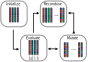
\includegraphics[width=88mm]{geneticAlgorithmFlowchart.pdf} 
	\caption{Genetic Algorithm Flowchart.}{The general process of how a genetic algorithm optimizes.}
	\label{fig:geneticFlowchart}
\end{figure}

Much like particle swarm, genetic algorithms have proven to be a powerful optimization approach that is much less susceptible to complex high-dimensional functions. In the next section I describe a set of experiments that utilize both optimization approaches to intelligently explore the neural response function.

 